\chapter{Experiment Modernization}
\label{chap:modernization}

The main experiment of the previous chapters runs part of its models and generators in \codename{R} and \codename{Java}, as \cref{chap:methodology_reassessment} describes, and its protocol carries the constraints of that environment. Its hyperparameter search penalizes the execution time and stops at a time limit, and its datasets have at most 10000 samples, because some of the models are too slow for an unrestricted search, \cref{subsec:hyperparameter_tuning}. The ranges of that search were set by hand, as values that seemed reasonable after a brief survey of the literature, as most of the works it cites also set theirs. \Cref{sec:mi_selection} found that the objective of the search observes too short a segment of the stream to recognize the configurations that are best in the long run, and that the search is itself a source of variation.

This chapter replaces the environment, the benchmark models and the hyperparameter selection, and repeats the main experiment under them. The model it evaluates is \MicroTEDAClusPlus as \cref{sec:mi_final_model} defines it, without changes.

\section{Environment}
\label{sec:mod_environment}

The experiment is written in \codename{Python} only. Its numerical parts run in compiled code through the libraries that provide them, and no other runtime is involved. \MicroTEDAClusPlus keeps the implementation of \cref{sec:mi_final_model}. Every model is used through one interface: it predicts the labels of a batch, learns the batch, and reports the number of structures of its summary of the stream, which generalizes the microcluster count of \cref{sec:evaluation_metrics}. A sample that a model predicts before it has any cluster is labelled as noise.

\subsection{Stream Generators}
\label{subsec:mod_generators}

Four generators of \cref{sec:datasets} ran in \codename{R}: that of \Cassini and those of \BenchmarkOne, \BenchmarkTwo and \RandomRBFGeneratorEvents, the last from MOA \cite{bifet2010moa} through \codename{streamMOA} \cite{streamMOA2024}. They are ported to \codename{Python}, following their reference implementations step by step. The Chameleon datasets remain the files of \cref{sec:datasets}, and the scalability streams were already generated in \codename{Python}. A stream is determined by its dataset and its run, which seed its generator.

Each port is compared with the streams that \codename{R} generated for the previous experiment, 126 streams of each source per dataset. For the three generators whose samples are independent given the time, the distributions of the samples are compared by Kolmogorov-Smirnov tests on each coordinate of each cluster and by a chi-squared test on the cluster proportions, \cref{tab:mod_generators_distribution}. The structure of the four streams is compared through descriptors computed in windows of 500 samples, \cref{tab:mod_generators_descriptors,fig:mod_generators_descriptors}, and the behaviour of three models with fixed hyperparameters through their ARI, \cref{tab:mod_generators_behaviour}. Descriptors and behaviour are compared by the Mann-Whitney test, with the Holm correction and the threshold on Cliff's delta of \cref{sec:statistical_significance}. No test finds a difference in the distributions of the samples, in the descriptors computed in windows, or in the behaviour of the models.

\begin{table}[htbp]
\centering
\small
\caption{Two-sample tests between the samples generated by R and by the port, pooled over the streams: Kolmogorov-Smirnov tests on each coordinate of each cluster and a chi-squared test on the cluster proportions.}
\adjustbox{max width=\textwidth, max totalheight=0.82\textheight}{%
\begin{tabular}{l c c c }
\toprule
Quantity & B1 & B2 & CSN \\
\midrule
Samples of each source & 504000 & 504000 & 504000 \\
Tests on the coordinates & 6 & 6 & 6 \\
Largest Kolmogorov-Smirnov statistic & 0.0054 & 0.0031 & 0.0051 \\
Smallest adjusted $p$-value of the coordinates & 1.00 & 1.00 & 0.32 \\
Adjusted $p$-value of the cluster proportions & 1.00 & 1.00 & 1.00 \\
\bottomrule
\end{tabular}
}
\label{tab:mod_generators_distribution}
\end{table}

\begin{table}[htbp]
\centering
\caption{Structure of the streams generated by R and by the port: medians over 126 streams. The clusters created are counted over the whole stream, and the other quantities are means over windows of 500 samples. A value in red is significantly different from that of R.}
\adjustbox{width=\textwidth, totalheight=0.82\textheight, keepaspectratio}{%
\begin{tabular}{l c c c c }
\toprule
Source & B1 & B2 & RBF & CSN \\
\midrule
\multicolumn{5}{l}{\textit{Clusters present}} \\
R & 2.00 & 3.00 & 3.25 & 3.00 \\
port & 2.00 & 3.00 & 3.17 & 3.00 \\
\midrule
\multicolumn{5}{l}{\textit{Share of noise}} \\
R & 0.090 & 0.000 & 0.243 & 0.000 \\
port & 0.091 & 0.000 & 0.230 & 0.000 \\
\midrule
\multicolumn{5}{l}{\textit{Spread of a cluster}} \\
R & 0.033 & 0.159 & 0.042 & 0.687 \\
port & 0.033 & 0.159 & 0.042 & 0.686 \\
\midrule
\multicolumn{5}{l}{\textit{Displacement of a cluster between windows}} \\
R & 0.103 & 0.123 & 0.047 & 0.065 \\
port & 0.103 & 0.123 & 0.047 & 0.063 \\
\midrule
\multicolumn{5}{l}{\textit{Smallest distance between clusters}} \\
R & 0.325 & 0.410 & 0.177 & 1.222 \\
port & 0.325 & 0.409 & 0.177 & 1.220 \\
\midrule
\multicolumn{5}{l}{\textit{Clusters created along the stream}} \\
R & 2.00 & 3.00 & 7.50 & 3.00 \\
port & 2.00 & 3.00 & \textcolor{red}{7.00} & 3.00 \\
\bottomrule
\end{tabular}
}
\label{tab:mod_generators_descriptors}
\end{table}


\begin{figure}[htbp]
    \centering
    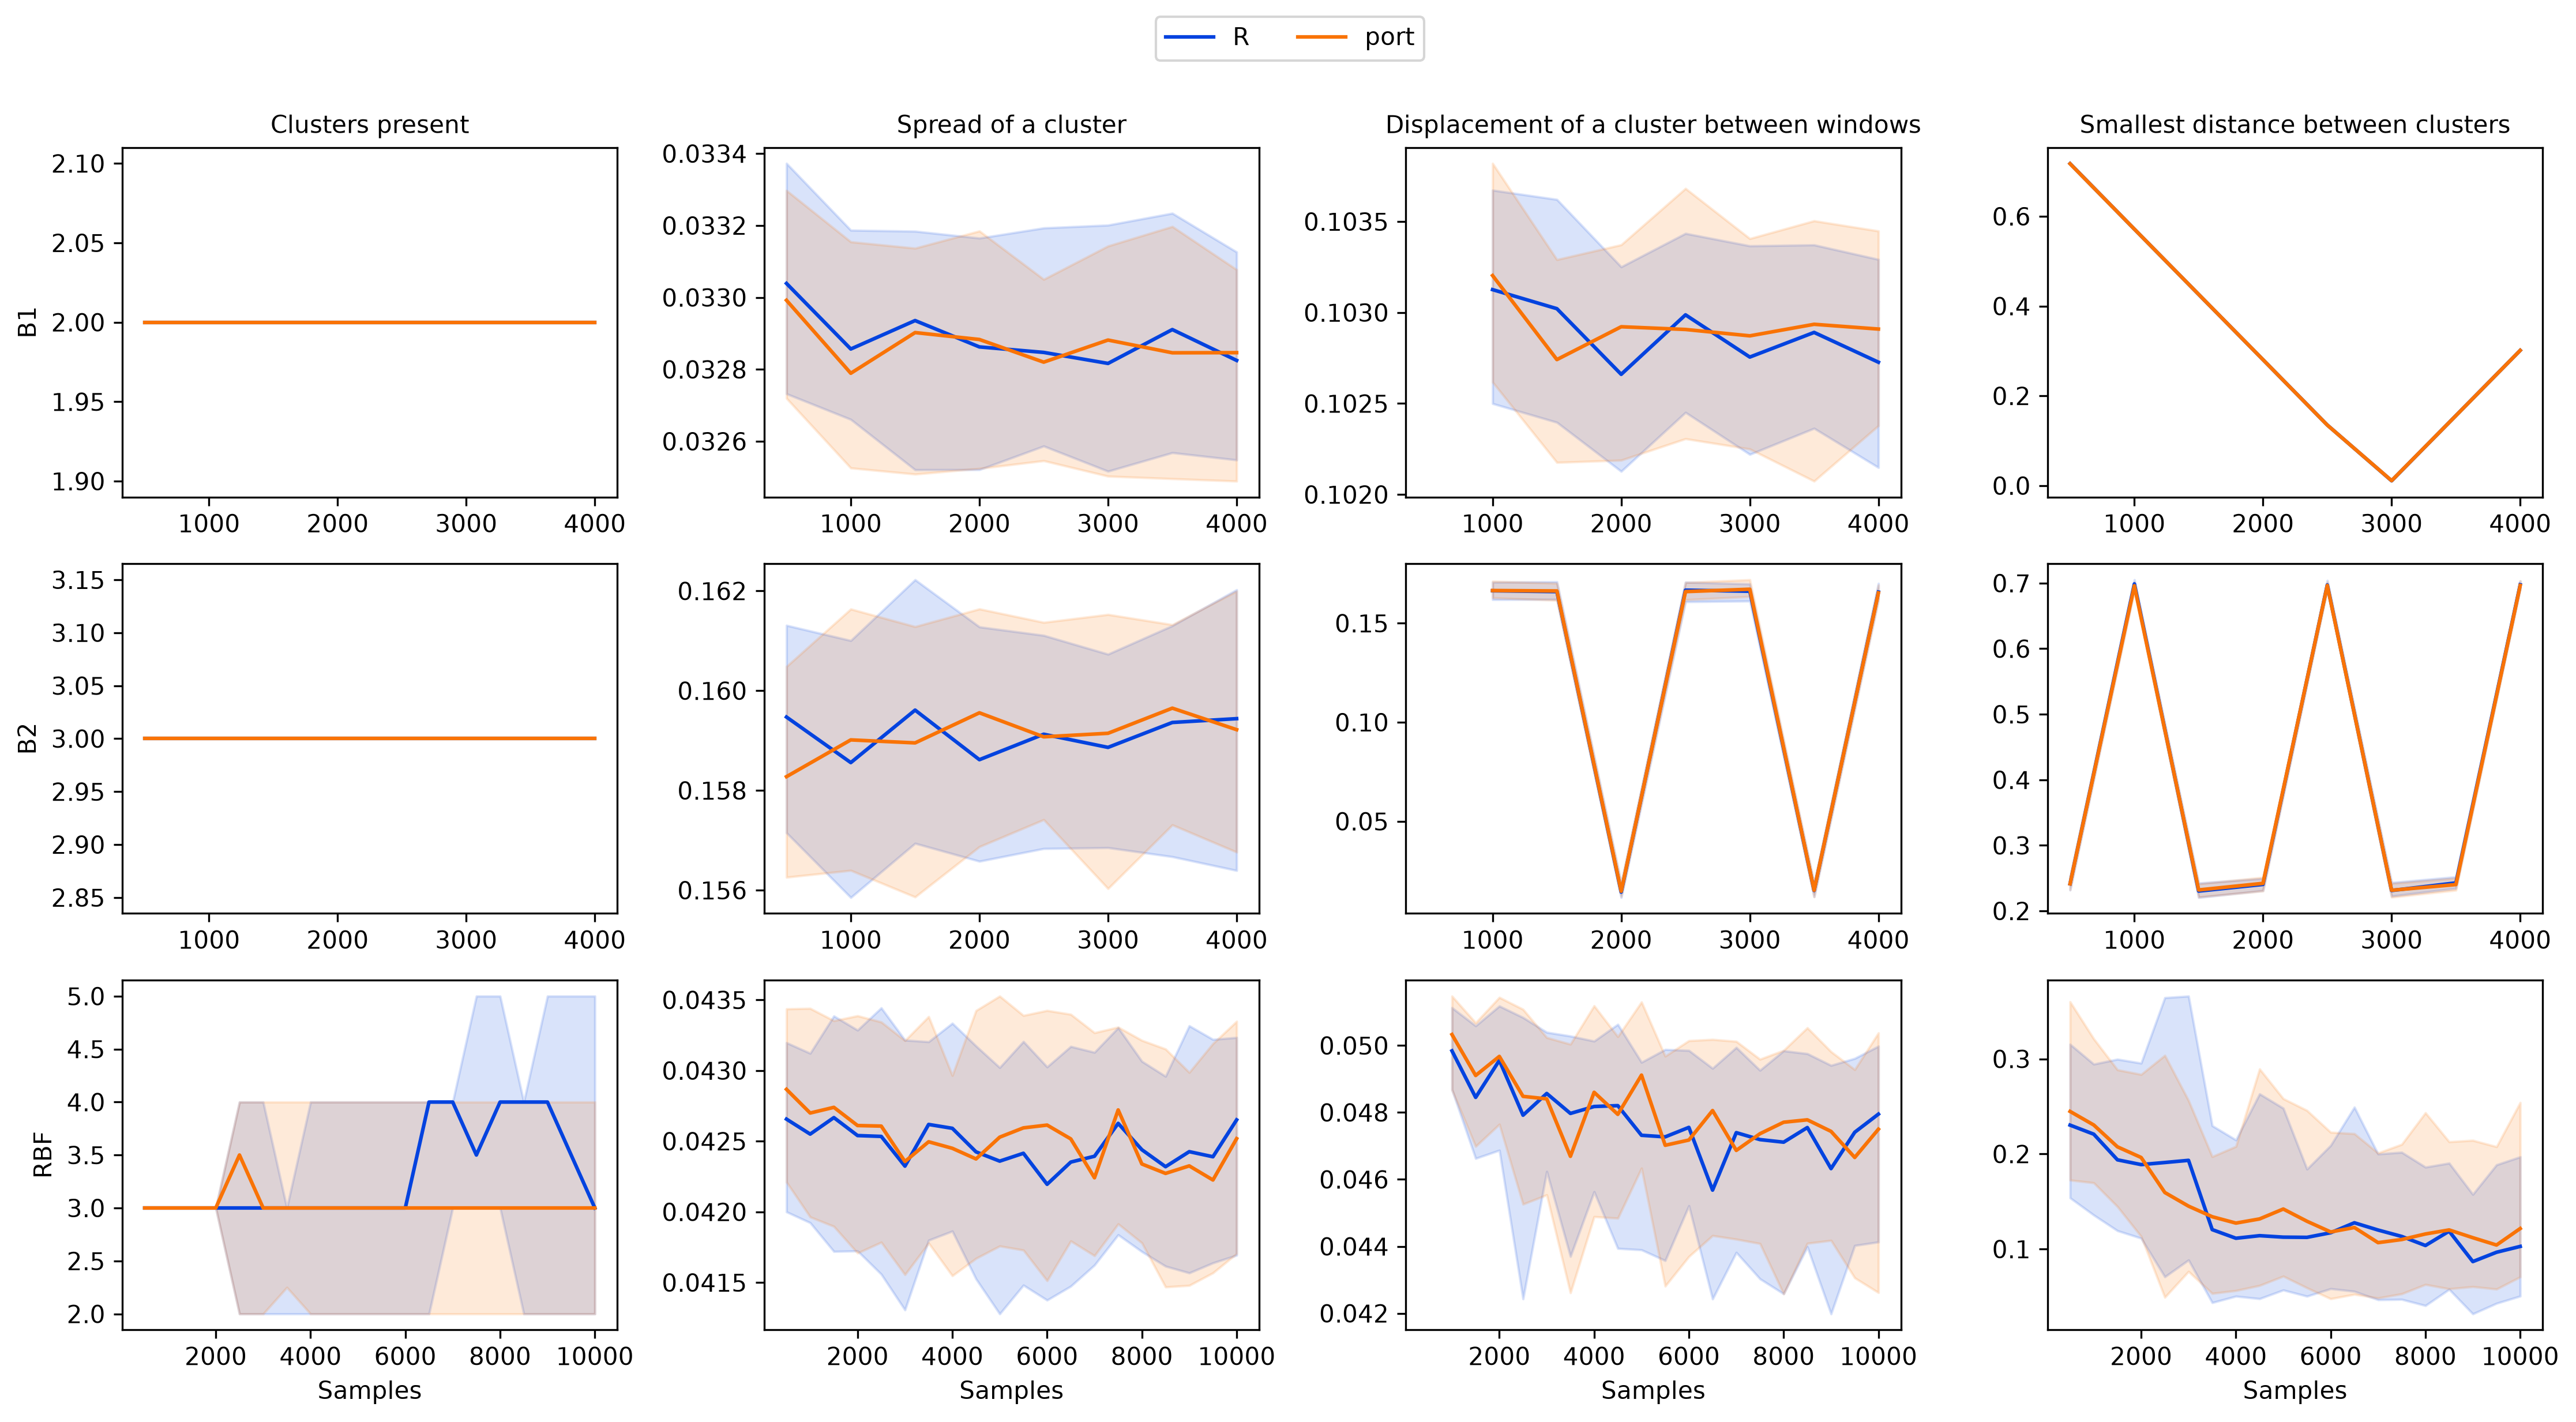
\includegraphics[width=\textwidth]{Modernization/artifacts/generators/plots/descriptors.png}
    \caption{Descriptors of the concept drift streams generated by \codename{R} and by the port, along the stream: medians and interquartile bands over the streams.}
    \label{fig:mod_generators_descriptors}
\end{figure}

\begin{table}[htbp]
\centering
\small
\caption[Models with fixed hyperparameters on the streams generated by R and by the port]{Models with fixed hyperparameters on the streams generated by R and by the port: medians over the streams. A value in red is significantly different from that of R.}
\adjustbox{max width=\textwidth, max totalheight=0.82\textheight}{%
\begin{tabular}{l c c c c }
\toprule
Model and source & B1 & B2 & RBF & CSN \\
\midrule
\multicolumn{5}{l}{\textit{Overall ARI}} \\
MicroTEDAClus+, R & 0.956 & 0.663 & 0.598 & 0.200 \\
MicroTEDAClus+, port & 0.953 & 0.666 & 0.617 & 0.197 \\
mini-batch k-means, R & 0.821 & 0.638 & 0.428 & 0.562 \\
mini-batch k-means, port & 0.816 & 0.647 & 0.431 & 0.540 \\
BIRCH, R & 0.132 & 0.691 & 0.377 & 1.000 \\
BIRCH, port & 0.133 & 0.688 & 0.366 & 1.000 \\
\midrule
\multicolumn{5}{l}{\textit{Steady-State ARI}} \\
MicroTEDAClus+, R & 0.973 & 0.783 & 0.599 & 0.171 \\
MicroTEDAClus+, port & 0.956 & 0.777 & 0.587 & 0.165 \\
mini-batch k-means, R & 0.832 & 0.832 & 0.376 & 0.571 \\
mini-batch k-means, port & 0.828 & 0.847 & 0.455 & 0.572 \\
BIRCH, R & 0.138 & 0.931 & 0.381 & 1.000 \\
BIRCH, port & 0.127 & 0.940 & 0.389 & 1.000 \\
\bottomrule
\end{tabular}
}
\label{tab:mod_generators_behaviour}
\end{table}


The interface through which the previous experiment generated \RandomRBFGeneratorEvents gives the noise the class value of the first cluster that the generator creates after the initial ones, so the samples of that cluster are labelled as noise. The port labels the noise apart from every cluster, and the comparisons above apply the labelling of the reference to both sources. \Cref{tab:mod_generators_rbf_noise} shows the share of samples labelled as noise along the stream under each labelling.

\begin{table}[htbp]
\centering
\small
\caption[Share of the samples of the Random RBF stream that carry the noise label]{Share of the samples of the Random RBF stream that carry the noise label, in consecutive blocks of 1000 samples: medians over the streams.}
\adjustbox{max width=\textwidth, max totalheight=0.82\textheight}{%
\begin{tabular}{l c c c c c c c c c c }
\toprule
Source & 1 & 2 & 3 & 4 & 5 & 6 & 7 & 8 & 9 & 10 \\
\midrule
R & 0.10 & 0.33 & 0.33 & 0.31 & 0.29 & 0.24 & 0.22 & 0.20 & 0.12 & 0.12 \\
port, labels of the R wrapper & 0.10 & 0.33 & 0.29 & 0.30 & 0.26 & 0.24 & 0.22 & 0.14 & 0.11 & 0.11 \\
port & 0.10 & 0.10 & 0.10 & 0.10 & 0.10 & 0.10 & 0.10 & 0.10 & 0.10 & 0.10 \\
\bottomrule
\end{tabular}
}
\label{tab:mod_generators_rbf_noise}
\end{table}


\subsection{Length and Order of the Streams}
\label{subsec:mod_streams}

The generated streams are five times longer than those of the previous experiment, and so are their tuning segments, in answer to \cref{sec:mi_selection}. The Chameleon files keep their size. The streams without concept drift, which are those of \Cassini, of the Chameleon datasets and of the scalability datasets, are shuffled anew in every run. Each run of a Chameleon dataset thus has a stream of its own, where in the previous experiment all its runs processed one same stream, \cref{subsec:mi_selection_consequences}. The concept drift streams keep their order, which carries the drift.

\section{Benchmark Models}
\label{sec:mod_models}

The benchmark models are chosen by three criteria: they are established in the literature of stream clustering, their implementations are maintained libraries that the experiment imports instead of copying, and they are fast enough to be tuned without a time limit. Five models are retained: \DenStream \cite{cao2006density} and \DBSTREAM \cite{hahsler2016dbstream}, from \codename{River} \cite{montiel2021river}; \BIRCH \cite{zhang1996birch} and \MiniBatchKMeans \cite{sculley2010webscale}, from \codename{scikit-learn} \cite{pedregosa2011scikit}; and \BICO \cite{fichtenberger2013bico}, from the \codename{bico} package. They summarize the stream by density-based microclusters that fade, \DenStream and \DBSTREAM, by a tree of cluster features, \BIRCH, by a coreset, \BICO, and by centroids, \MiniBatchKMeans. This set replaces that of \cref{chap:results}.

\Cref{tab:mod_hyperparameters} lists the hyperparameters that the search selects for each model. A parameter is searched if it is part of the clustering method, and keeps the default of its library if it only sets a unit of time or the shape of a data structure. \DenStream and \DBSTREAM forget at a rate that is searched as its half-life, in samples. The outlier threshold $\beta\mu$ of \DenStream, which its formulation requires to exceed one, is searched as its position between one and $\mu$.

\begin{table}[htbp]
\centering
\small
\caption[Hyperparameters of the models and their categories]{Hyperparameters that the search selects for each model, and the category that gives each its range.}
\adjustbox{max width=\textwidth, max totalheight=0.82\textheight}{%
\begin{tabular}{l l l}
\toprule
Model & Hyperparameter & Category \\
\midrule
\modelname{MicroTEDAClus+} & \texttt{variance\_limit} & Relative variance \\
 & \texttt{decay} & Horizon \\
 & \texttt{noise\_distance} & Multiplier \\
\midrule
\modelname{DenStream} & \texttt{epsilon} & Distance \\
 & \texttt{half\_life} & Horizon \\
 & \texttt{mu} & Minimum points \\
 & \texttt{outlier\_ratio} & Ratio \\
 & \texttt{n\_samples\_init} & Horizon \\
\midrule
\modelname{DBSTREAM} & \texttt{clustering\_threshold} & Distance \\
 & \texttt{half\_life} & Horizon \\
 & \texttt{cleanup\_interval} & Horizon \\
 & \texttt{intersection\_factor} & Ratio \\
 & \texttt{minimum\_weight} & Minimum points \\
\midrule
\modelname{BIRCH} & \texttt{threshold} & Distance \\
 & \texttt{n\_clusters} & Clusters \\
\midrule
\modelname{Mini-batch k-means} & \texttt{n\_clusters} & Clusters \\
 & \texttt{reassignment\_ratio} & Ratio \\
\midrule
\modelname{BICO} & \texttt{n\_clusters} & Clusters \\
 & \texttt{summary\_size} & Summary size \\
\bottomrule
\end{tabular}
}
\label{tab:mod_hyperparameters}
\end{table}


\section{Hyperparameter Selection}
\label{sec:mod_selection}

The search remains the Bayesian optimization of \cref{subsec:hyperparameter_tuning} on the first 20\% of each stream, and the selected model is evaluated prequentially on the rest. Three things change: where the ranges come from, what the objective measures, and what bounds the search.

\subsection{Ranges by Rule}
\label{subsec:mod_ranges}

Each hyperparameter belongs to a kind, given in \cref{tab:mod_hyperparameters}, and each kind has one rule that computes its range from the tuning segment, given in \cref{tab:mod_rules}. A rule uses only what a deployment of the model also has before the stream continues: the samples of the segment and their labels. Below the median distance from a sample to its nearest neighbour, a structure of that radius holds a single sample, and above the median distance between two samples it holds half of the segment, so the distances of the rules span the scales at which a structure can summarize the data. The longest horizon is the length of the segment, the longest that the segment can tell apart from not forgetting at all. The rules replace ranges set by hand, which \cref{tab:mi_search_range_selection} showed to depend on the scale of the data. \Cref{tab:mod_ranges} gives the ranges that they produce in each dataset.

\begin{table}[htbp]
\centering
\caption{Rule of each kind of hyperparameter, for a tuning segment of $n$ samples with $k$ labelled clusters. Horizons, summary sizes, minimum points and numbers of clusters are integers.}
\begin{tabular}{p{0.16\textwidth} p{0.29\textwidth} p{0.29\textwidth} l}
\toprule
Kind & Lower end & Upper end & Scale \\
\midrule
Distance & median distance from a sample to its nearest neighbour & median distance between two samples & logarithmic \\
Relative variance & square of the lower distance, as a fraction of the total variance & square of the upper distance, as a fraction of the total variance & logarithmic \\
Horizon & $n/100$ samples & $n$ samples & logarithmic \\
Summary size & $2k$ & $n/4$ & logarithmic \\
Minimum points & $2$ & $\sqrt{n}$ & logarithmic \\
Ratio & $0.01$ & $0.99$ & linear \\
Multiplier & $1$ & $10$ & linear \\
Clusters & $2$ & $2k$ & linear \\
\bottomrule
\end{tabular}
\label{tab:mod_rules}
\end{table}

\begin{table}[htbp]
\centering
\small
\caption[Search ranges that the rules give]{Search ranges that the rules give to each category of hyperparameter: medians over 94 runs of the two ends of each range.}
\adjustbox{max width=\textwidth, max totalheight=0.82\textheight}{%
\begin{tabular}{l c c c c c c }
\toprule
Dataset & Distance & Relative variance & Horizon & Summary size & Minimum points & Clusters \\
\midrule
B1 & $2.1 \times 10^{-4}$ to 3.3 & $5.5 \times 10^{-7}$ to 138 & 4 to 4000 & 4 to 1000 & 1 to 63 & 2 to 40 \\
B2 & $5.3 \times 10^{-4}$ to 6.5 & $7.0 \times 10^{-7}$ to 106 & 4 to 4000 & 6 to 1000 & 1 to 63 & 2 to 60 \\
RBF & $2.5 \times 10^{-4}$ to 3.2 & $7.8 \times 10^{-7}$ to 136 & 10 to 10000 & 16 to 2500 & 1 to 100 & 2 to 100 \\
CSN & 0.002 to 16 & $2.2 \times 10^{-6}$ to 142 & 4 to 4000 & 6 to 1000 & 1 to 63 & 2 to 60 \\
DS3 & 0.44 to 2802 & $3.5 \times 10^{-6}$ to 146 & 2 to 2000 & 18 to 500 & 1 to 45 & 2 to 100 \\
DS4 & 0.48 to 2598 & $4.9 \times 10^{-6}$ to 143 & 2 to 1600 & 16 to 400 & 1 to 40 & 2 to 100 \\
S1 & $4.9 \times 10^{-5}$ to 30 & $1.2 \times 10^{-10}$ to 65 & 5 to 4400 & 6 to 1100 & 1 to 66 & 2 to 60 \\
S2 & 0.0026 to 60 & $1.8 \times 10^{-7}$ to 106 & 5 to 4400 & 6 to 1100 & 1 to 66 & 2 to 60 \\
S4 & 0.021 to 113 & $4.9 \times 10^{-6}$ to 167 & 5 to 4400 & 6 to 1100 & 1 to 66 & 2 to 60 \\
S8 & 0.067 to 195 & $2.5 \times 10^{-5}$ to 216 & 5 to 4400 & 6 to 1100 & 1 to 66 & 2 to 60 \\
S16 & 0.15 to 285 & $6.0 \times 10^{-5}$ to 230 & 5 to 4400 & 6 to 1100 & 1 to 66 & 2 to 60 \\
S32 & 0.26 to 419 & $9.7 \times 10^{-5}$ to 252 & 5 to 4400 & 6 to 1100 & 1 to 66 & 2 to 60 \\
S64 & 0.43 to 612 & $1.3 \times 10^{-4}$ to 270 & 5 to 4400 & 6 to 1100 & 1 to 66 & 2 to 60 \\
\bottomrule
\end{tabular}
}
\label{tab:mod_ranges}
\end{table}


\subsection{Objective and Search}
\label{subsec:mod_objective}

The objective is the median of the batch ARI over the second half of the tuning segment. It is the quantity that the Overall ARI reports, computed after the configuration has had the first half of the segment to form its summary, which addresses the slow maturation shown in \cref{tab:mi_selection_maturation}. It has no term of execution time.

Every model receives 100 trials, without a time limit. The search of a task is seeded by its dataset, its model and its run, and its objective involves no measurement of time, so the selection depends neither on the speed of the machine nor on its load. To measure what the change of protocol does, \MicroTEDAClusPlus is also tuned by the previous protocol of \cref{subsec:hyperparameter_tuning}, with its previous ranges, on the same streams.

\section{Execution and Measurements}
\label{sec:mod_measurements}

A task is a dataset, a model and a run, and the experiment executes the tasks of 94 runs, 13 datasets and the six models in parallel processes. Parallel execution disturbs the execution time, so time is measured in a separate pass: the tasks of the first ten runs are evaluated again, one at a time, with their selected hyperparameters, three times each, and the fastest evaluation is kept.

Memory is measured in another pass, over every task, by tracking every allocation of the process with \codename{memray} \cite{memray}, which counts the memory allocated by compiled code as well as that allocated by \codename{Python}. Two quantities are kept: the memory still allocated when the stream ends, which is what the model holds, and the peak during the evaluation, which adds the working memory of its steps. Each task is first evaluated without tracking, so that what is created on first use is in place, and then tracked three times, of which the smallest values are kept. These quantities are not comparable with the memory reported in the previous chapters, which counted only the \codename{Python} objects of a model.

The results are compared by the analysis of \cref{sec:statistical_significance}, as in \cref{chap:results}: a value in bold is statistically indistinguishable from the best model of its dataset, and a value in red from the worst. The tables refer to the datasets by the abbreviations of \cref{tab:mi_dataset_abbreviations}, and to \datasetname{SCL-$d$} as S$d$.

\section{Results}
\label{sec:mod_results}

\subsection{Clustering Quality}
\label{subsec:mod_quality}

\begin{table}[htbp]
\centering
\small
\caption[Clustering quality of \modelname{MicroTEDAClus+} and the benchmark models]{Clustering quality of \modelname{MicroTEDAClus+} and the benchmark models: medians over 94 runs.}
\adjustbox{max width=\textwidth, max totalheight=0.82\textheight}{%
\begin{tabular}{l c c c c c c }
\toprule
Model & B1 & B2 & RBF & CSN & DS3 & DS4 \\
\midrule
\multicolumn{7}{l}{\textit{Overall ARI}} \\
\modelname{MicroTEDAClus+} & 0.889 & 0.599 & 0.653 & 0.916 & 0.347 & 0.378 \\
Better/same/worse & 5/0/0 & 0/0/5 & 1/1/3 & 4/1/0 & 0/4/1 & 2/3/0 \\
\modelname{DenStream} & \textbf{0.829} & \textcolor{red}{0.625} & 0.605 & \textbf{0.637} & 0.381 & \textbf{0.354} \\
\modelname{DBSTREAM} & \textbf{0.852} & \textcolor{red}{0.825} & \textcolor{red}{0.664} & \textbf{0.758} & 0.371 & \textbf{0.354} \\
\modelname{BIRCH} & \textbf{0.821} & \textcolor{red}{0.673} & \textcolor{red}{0.690} & 1.000 & 0.356 & 0.378 \\
\modelname{Mini-batch k-means} & \textbf{0.863} & \textcolor{red}{0.642} & \textbf{0.587} & \textbf{0.588} & 0.377 & 0.366 \\
\modelname{BICO} & \textbf{0.876} & \textcolor{red}{0.774} & \textcolor{red}{0.681} & \textbf{0.595} & \textcolor{red}{0.409} & 0.371 \\
\midrule
\multicolumn{7}{l}{\textit{Steady-State ARI}} \\
\modelname{MicroTEDAClus+} & 0.790 & 0.567 & 0.466 & 0.792 & 0.348 & 0.367 \\
Better/same/worse & 4/1/0 & 0/0/5 & 0/0/5 & 2/2/1 & 0/4/1 & 0/5/0 \\
\modelname{DenStream} & \textbf{0.718} & \textcolor{red}{0.637} & \textcolor{red}{0.621} & 0.686 & 0.380 & 0.354 \\
\modelname{DBSTREAM} & 0.859 & \textcolor{red}{0.790} & \textcolor{red}{0.760} & 0.786 & 0.362 & 0.352 \\
\modelname{BIRCH} & \textbf{0.136} & \textcolor{red}{0.714} & \textcolor{red}{0.677} & \textcolor{red}{1.000} & 0.378 & 0.365 \\
\modelname{Mini-batch k-means} & \textbf{0.611} & \textcolor{red}{0.663} & \textcolor{red}{0.609} & \textbf{0.599} & 0.391 & 0.356 \\
\modelname{BICO} & \textbf{0.180} & \textcolor{red}{0.758} & \textcolor{red}{0.718} & \textbf{0.596} & \textcolor{red}{0.406} & 0.359 \\
\bottomrule
\end{tabular}
}
\label{tab:mod_quality}
\end{table}


In the Overall ARI, \cref{tab:mod_quality}, \MicroTEDAClusPlus is indistinguishable from the best model in \BenchmarkOne, \Cassini and \ChameleonDSFour, and from the worst in \BenchmarkTwo and \ChameleonDSThree. At the penultimate batch, \DBSTREAM is indistinguishable from the best model in the three concept drift datasets, and \MicroTEDAClusPlus in \BenchmarkOne only. At the fifth batch, \MicroTEDAClusPlus is indistinguishable from the best model in the three concept drift datasets and from the worst in the three static ones.

In \BenchmarkOne, \BIRCH and \BICO have the largest drops of the table and the lowest scores at the penultimate batch. Neither of them forgets, and the clusters of that stream move.

\begin{table}[htbp]
\centering
\caption{Quality of the models along the dimension of the data: medians over 94 runs. A value in bold is statistically indistinguishable from the best model of its dataset, and a value in red from the worst.}
\adjustbox{width=\textwidth, totalheight=0.82\textheight, keepaspectratio}{%
\begin{tabular}{l c c c c c c c }
\toprule
Model & S1 & S2 & S4 & S8 & S16 & S32 & S64 \\
\midrule
\multicolumn{8}{l}{\textit{Overall ARI}} \\
\modelname{MicroTEDAClus+} & \textcolor{red}{0.719} & \textbf{0.938} & \textbf{1.000} & \textbf{1.000} & \textbf{1.000} & \textbf{1.000} & \textbf{1.000} \\
\modelname{DenStream} & 0.780 & 0.885 & 0.961 & 0.968 & \textcolor{red}{0.978} & \textcolor{red}{0.991} & 1.000 \\
\modelname{DBSTREAM} & \textbf{0.776} & 0.928 & 0.966 & 0.975 & \textcolor{red}{0.975} & \textcolor{red}{0.982} & 0.986 \\
\modelname{BIRCH} & \textbf{0.806} & 0.923 & 0.951 & 1.000 & \textbf{1.000} & 1.000 & \textcolor{red}{0.895} \\
\modelname{Mini-batch k-means} & \textbf{0.779} & \textcolor{red}{0.855} & \textcolor{red}{0.901} & \textcolor{red}{0.948} & \textcolor{red}{0.981} & 1.000 & 1.000 \\
\modelname{BICO} & \textbf{0.800} & 0.891 & 0.940 & 0.963 & 0.982 & \textbf{1.000} & 1.000 \\
\midrule
\multicolumn{8}{l}{\textit{Steady-State ARI}} \\
\modelname{MicroTEDAClus+} & \textcolor{red}{0.698} & \textbf{0.925} & \textbf{0.998} & \textbf{1.000} & \textbf{1.000} & \textbf{1.000} & \textbf{1.000} \\
\modelname{DenStream} & 0.748 & 0.875 & 0.957 & 0.968 & \textcolor{red}{0.972} & \textcolor{red}{0.999} & 1.000 \\
\modelname{DBSTREAM} & \textbf{0.776} & \textbf{0.917} & 0.971 & 0.974 & \textcolor{red}{0.972} & \textcolor{red}{0.981} & 0.984 \\
\modelname{BIRCH} & \textbf{0.792} & \textbf{0.913} & 0.954 & 1.000 & \textbf{1.000} & 1.000 & \textcolor{red}{0.881} \\
\modelname{Mini-batch k-means} & \textbf{0.795} & \textcolor{red}{0.849} & \textcolor{red}{0.902} & \textcolor{red}{0.946} & 0.982 & 1.000 & \textbf{1.000} \\
\modelname{BICO} & \textbf{0.758} & 0.888 & 0.933 & 0.965 & 0.983 & \textbf{1.000} & \textbf{1.000} \\
\bottomrule
\end{tabular}
}
\label{tab:mod_scalability}
\end{table}


\begin{figure}[htbp]
    \centering
    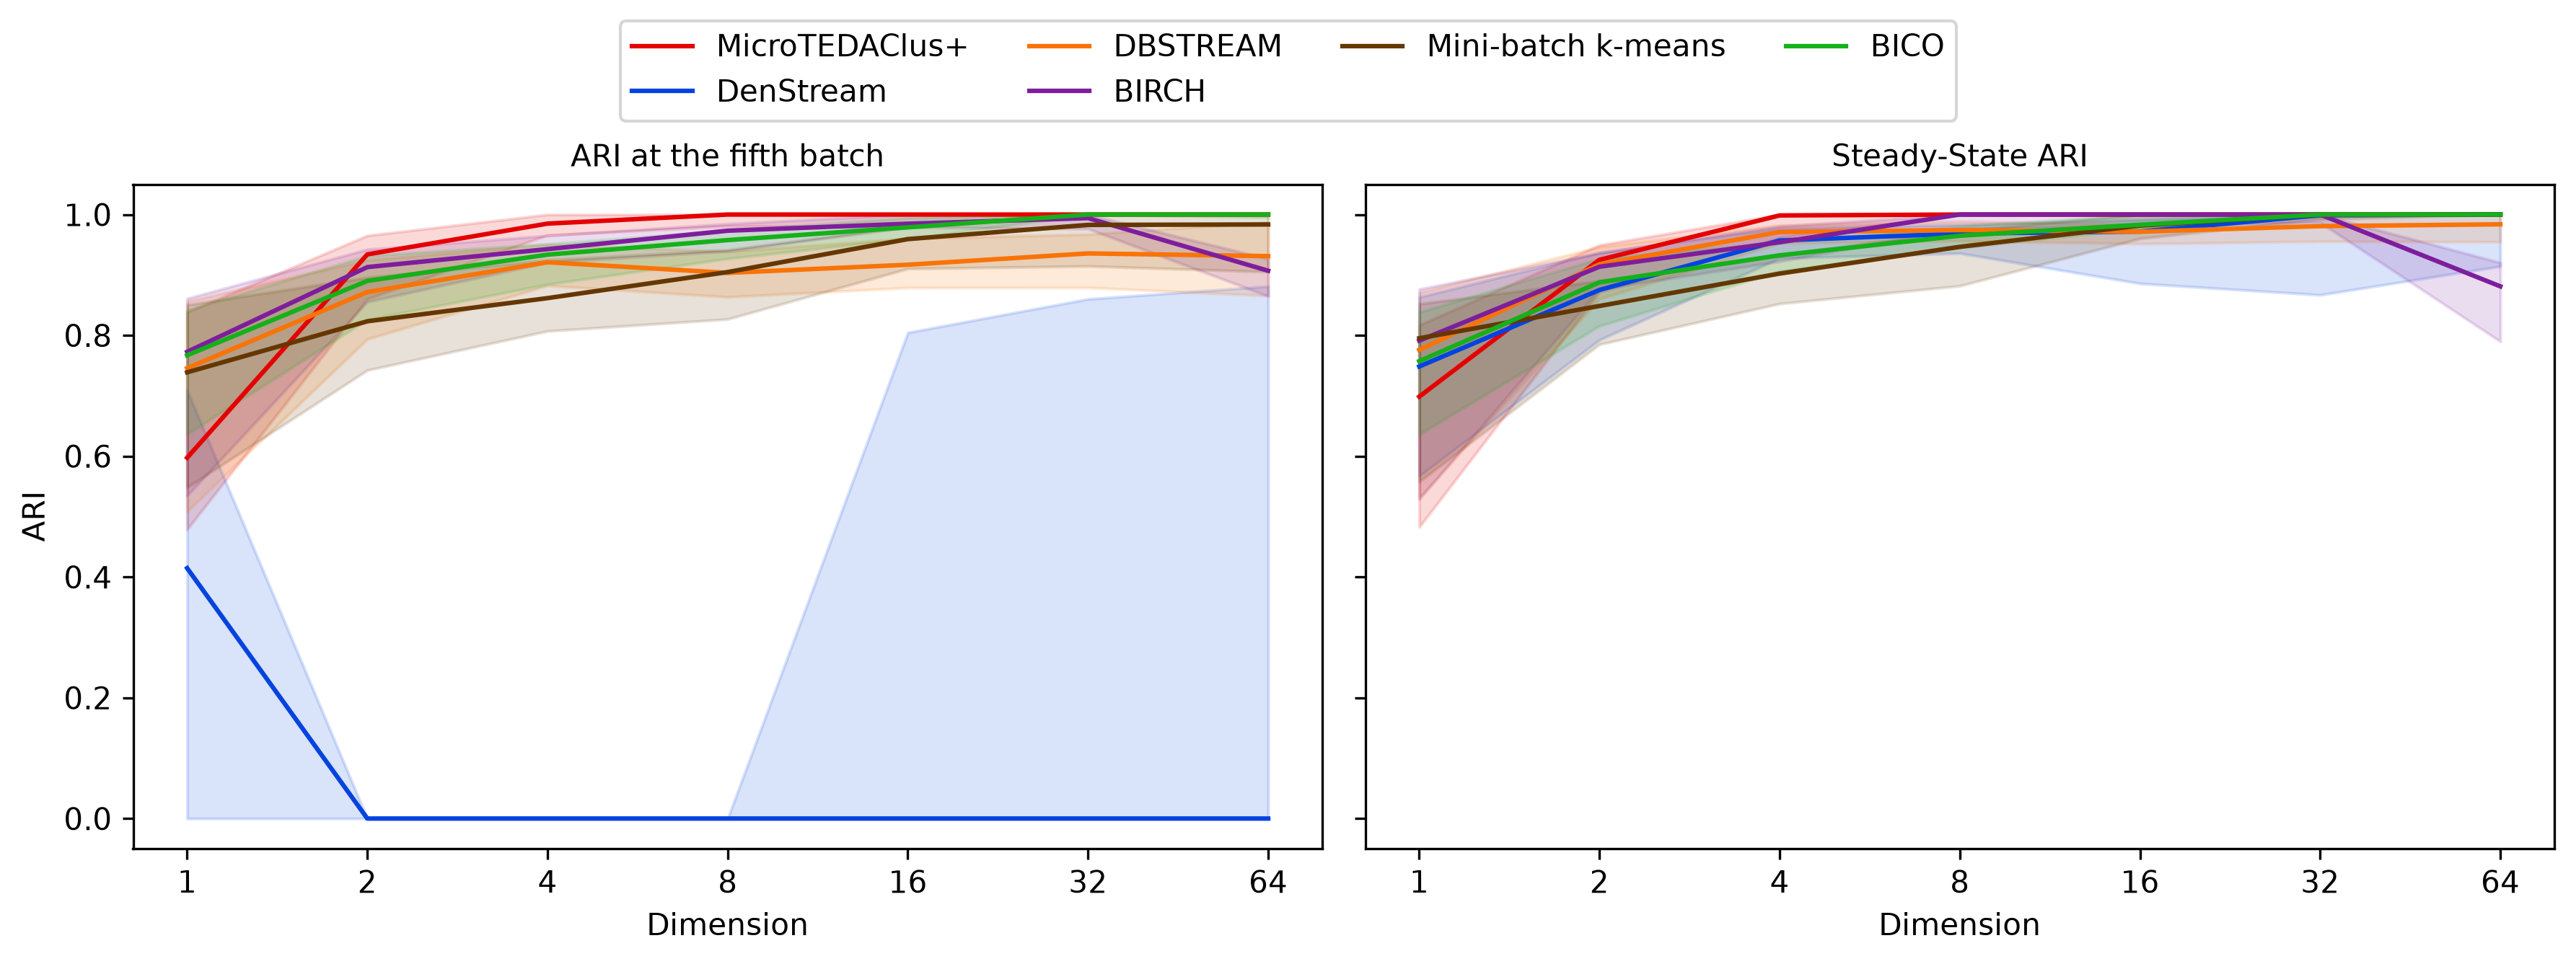
\includegraphics[width=\textwidth]{Modernization/artifacts/experiment/plots/dimension_scalability.png}
    \caption{ARI at the fifth batch, at left, and at the penultimate batch, at right, against the dimension of the scalability streams: medians and interquartile bands over 94 runs.}
    \label{fig:mod_dimension}
\end{figure}

In the scalability streams, \cref{tab:mod_scalability,fig:mod_dimension}, \MicroTEDAClusPlus is indistinguishable from the best model from two dimensions on, in both metrics, and from the worst with one dimension. \BIRCH, among the best with sixteen dimensions, is among the worst with sixty-four, where its score varies widely along the stream, \cref{fig:mod_stream}.

\begin{figure}[htbp]
    \centering
    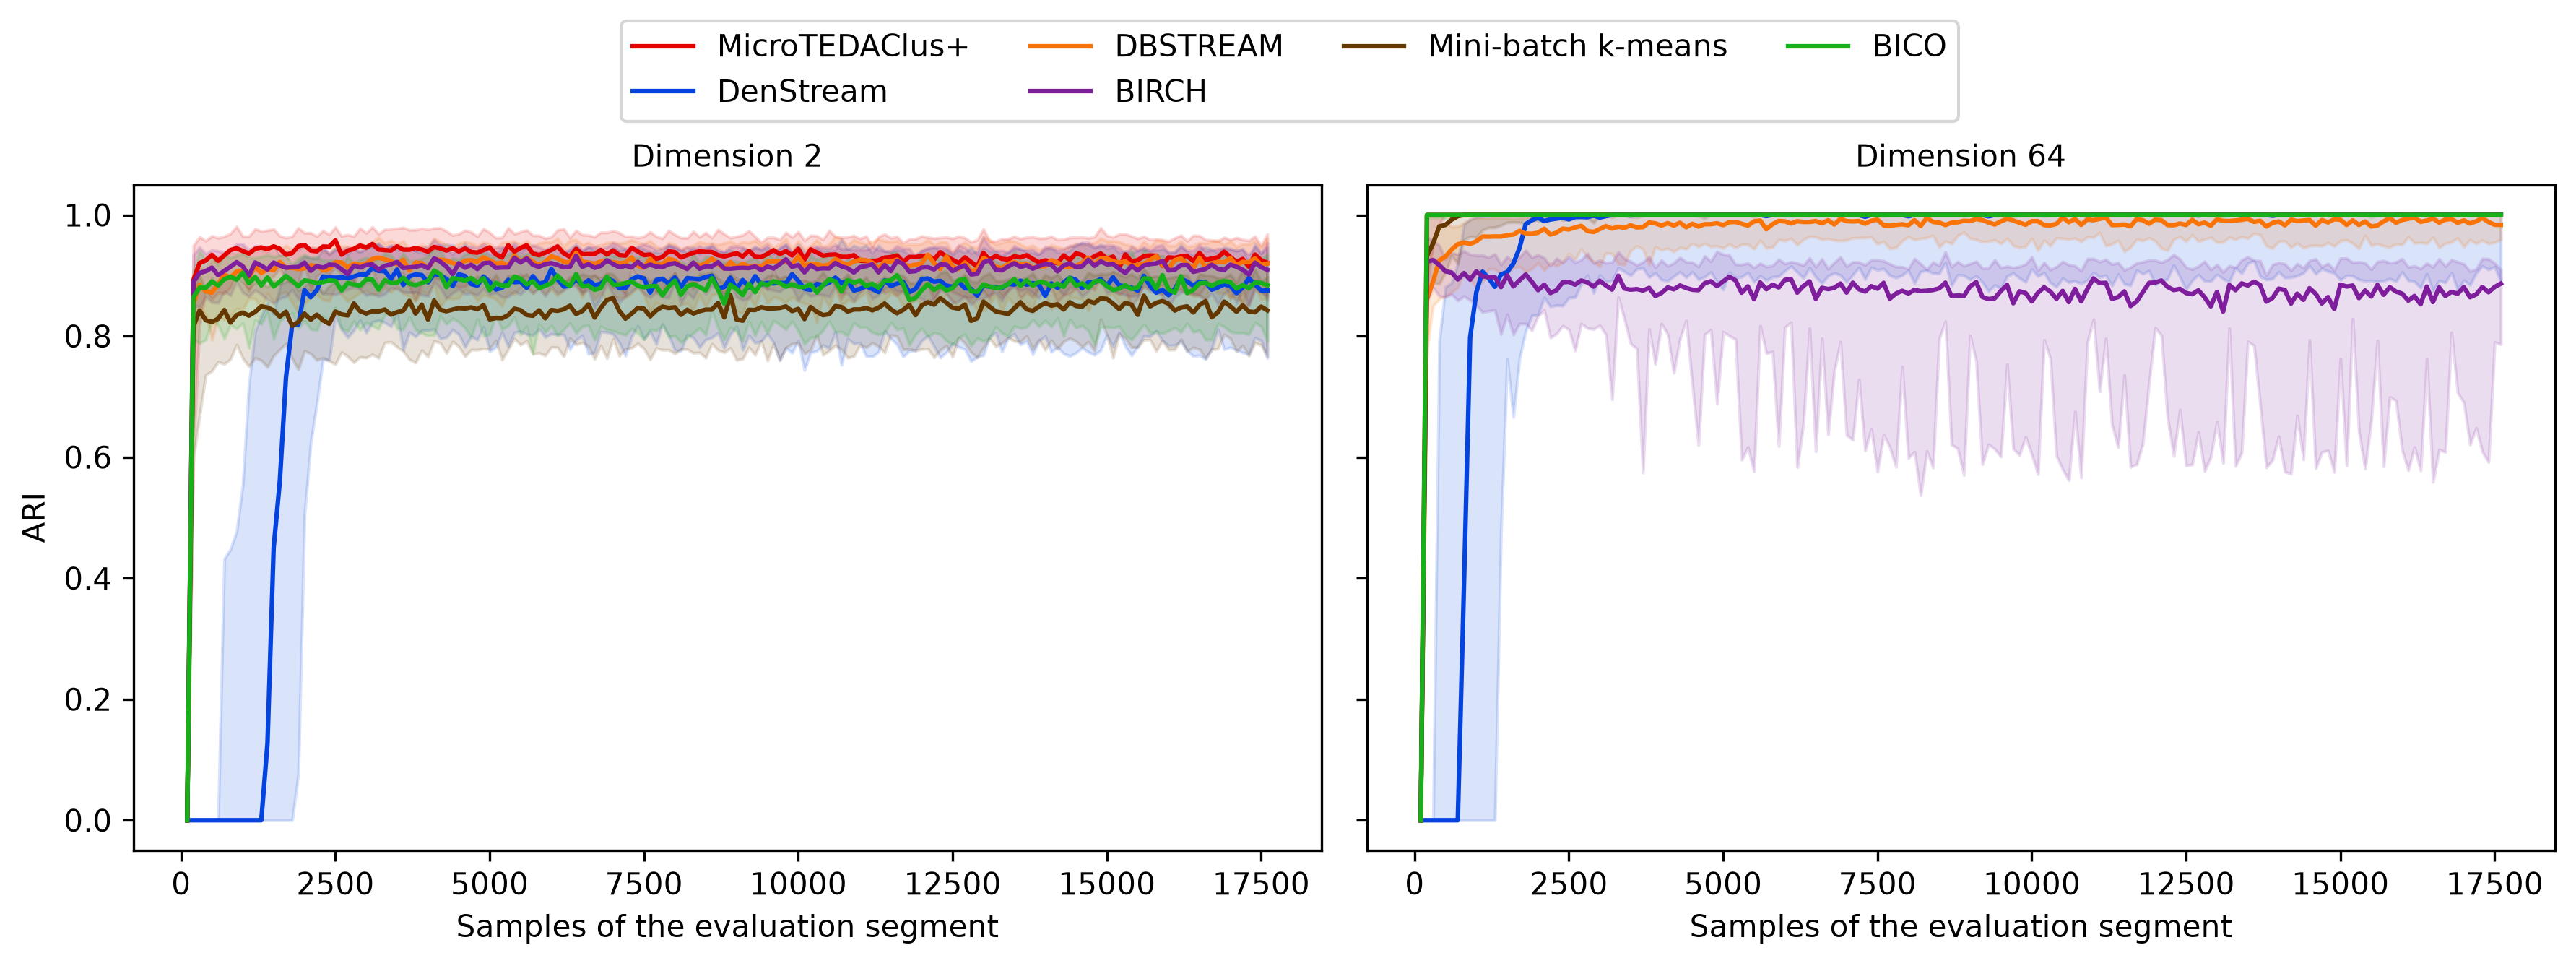
\includegraphics[width=\textwidth]{Modernization/artifacts/experiment/plots/stream_scalability.png}
    \caption{Batch ARI along the evaluation segment of \datasetname{SCL-2}, at left, and of \datasetname{SCL-64}, at right: medians and interquartile bands over 94 runs.}
    \label{fig:mod_stream}
\end{figure}

\DenStream scores zero at the fifth batch in the concept drift datasets, \cref{tab:mod_quality}, and from two dimensions on, \cref{fig:mod_dimension}. \Cref{fig:mod_stream} shows why: it labels every sample as noise until its initialization buffer is full, and the search selects long buffers. The objective scores only the second half of the tuning segment, where a late start costs nothing, while the Overall ARI counts the whole stream. This disagreement between the objective and the reported metric is a limitation of the protocol, not of the model, and the experiment was not repeated without it.

\subsection{The Change of Protocol}
\label{subsec:mod_protocols}

\begin{table}[htbp]
\centering
\small
\caption[\MicroTEDAClusPlus{} under the two protocols of hyperparameter selection]{\MicroTEDAClusPlus{} with its hyperparameters selected by the previous protocol and by the protocol by rules, on the same streams: medians over 94 runs.}
\adjustbox{max width=\textwidth, max totalheight=0.82\textheight}{%
\begin{tabular}{l c c c c c c c c c c c c c }
\toprule
Selection & B1 & B2 & RBF & CSN & DS3 & DS4 & S1 & S2 & S4 & S8 & S16 & S32 & S64 \\
\midrule
\multicolumn{14}{l}{\textit{Overall ARI}} \\
Previous protocol & 0.897 & 0.605 & 0.573 & 0.607 & 0.295 & 0.345 & 0.702 & 0.942 & 1.000 & 1.000 & 1.000 & 1.000 & 1.000 \\
Protocol by rules & 0.889 & \textcolor{red}{0.599} & \textbf{0.653} & \textbf{0.916} & \textbf{0.347} & \textbf{0.378} & 0.719 & 0.938 & 1.000 & 1.000 & 1.000 & \textbf{1.000} & \textbf{1.000} \\
\midrule
\multicolumn{14}{l}{\textit{Steady-State ARI}} \\
Previous protocol & 0.223 & 0.573 & 0.215 & 0.421 & 0.279 & 0.324 & 0.595 & 0.924 & 0.998 & 1.000 & 1.000 & 1.000 & 1.000 \\
Protocol by rules & \textbf{0.790} & 0.567 & 0.466 & \textbf{0.792} & \textbf{0.348} & \textbf{0.367} & 0.698 & 0.925 & 0.998 & 1.000 & 1.000 & \textbf{1.000} & 1.000 \\
\bottomrule
\end{tabular}
}
\label{tab:mod_protocols}
\end{table}


\Cref{tab:mod_protocols} compares \MicroTEDAClusPlus under the two protocols on the same streams. The protocol by rules raises its Overall ARI in six datasets and lowers it in \BenchmarkTwo, and raises its Steady-State ARI in five datasets without lowering it in any. The largest differences are at the penultimate batch of \BenchmarkOne and \Cassini. This agrees with \cref{subsec:mi_selection_consequences}, which located the most direct improvement of the model in the selection of its hyperparameters rather than in its algorithm.

\subsection{Selected Hyperparameters}
\label{subsec:mod_selected}

\begin{table}[htbp]
\centering
\small
\caption[Selected values at the ends of their search ranges]{Percentage of the 94 runs in which the selected value of a hyperparameter lies within a twentieth of the width of its search range from one of its ends, in the scale of the search.}
\adjustbox{max width=\textwidth, max totalheight=0.82\textheight}{%
\begin{tabular}{l c c c c c c c c c c c c c }
\toprule
Model and hyperparameter & B1 & B2 & RBF & CSN & DS3 & DS4 & S1 & S2 & S4 & S8 & S16 & S32 & S64 \\
\midrule
\multicolumn{14}{l}{\textit{At the lower end}} \\
\modelname{MicroTEDAClus+}, \texttt{variance\_limit} & 0 & 0 & 0 & 0 & 0 & 0 & 0 & 0 & 6 & 13 & 4 & 6 & 3 \\
\modelname{MicroTEDAClus+}, \texttt{decay} & 31 & 13 & 16 & 0 & 4 & 3 & 3 & 1 & 5 & 2 & 3 & 2 & 4 \\
\modelname{MicroTEDAClus+}, \texttt{noise\_distance} & 0 & 0 & 0 & 0 & 0 & 0 & 0 & 0 & 0 & 0 & 2 & 0 & 3 \\
\modelname{DenStream}, \texttt{epsilon} & 7 & 2 & 0 & 0 & 0 & 2 & 0 & 3 & 0 & 0 & 1 & 1 & 1 \\
\modelname{DenStream}, \texttt{half\_life} & 0 & 1 & 6 & 0 & 2 & 9 & 2 & 1 & 1 & 1 & 7 & 7 & 4 \\
\modelname{DenStream}, \texttt{mu} & 46 & 4 & 18 & 1 & 17 & 14 & 21 & 29 & 69 & 52 & 18 & 15 & 14 \\
\modelname{DenStream}, \texttt{outlier\_ratio} & 6 & 10 & 4 & 6 & 3 & 3 & 7 & 6 & 3 & 4 & 4 & 5 & 5 \\
\modelname{DenStream}, \texttt{n\_samples\_init} & 0 & 3 & 1 & 13 & 0 & 1 & 3 & 3 & 0 & 1 & 1 & 0 & 1 \\
\modelname{DBSTREAM}, \texttt{clustering\_threshold} & 0 & 0 & 0 & 0 & 0 & 0 & 0 & 0 & 0 & 0 & 0 & 0 & 1 \\
\modelname{DBSTREAM}, \texttt{half\_life} & 0 & 3 & 19 & 1 & 3 & 3 & 5 & 1 & 0 & 0 & 0 & 0 & 3 \\
\modelname{DBSTREAM}, \texttt{cleanup\_interval} & 6 & 3 & 4 & 2 & 4 & 5 & 6 & 2 & 2 & 3 & 5 & 5 & 5 \\
\modelname{DBSTREAM}, \texttt{intersection\_factor} & 3 & 0 & 2 & 1 & 2 & 5 & 6 & 5 & 2 & 1 & 1 & 7 & 2 \\
\modelname{DBSTREAM}, \texttt{minimum\_weight} & 19 & 13 & 27 & 11 & 18 & 15 & 13 & 32 & 50 & 44 & 40 & 18 & 15 \\
\modelname{BIRCH}, \texttt{threshold} & 1 & 3 & 16 & 6 & 6 & 7 & 9 & 23 & 51 & 70 & 73 & 90 & 9 \\
\modelname{BIRCH}, \texttt{n\_clusters} & 16 & 0 & 0 & 0 & 0 & 0 & 3 & 0 & 0 & 0 & 0 & 0 & 0 \\
\modelname{Mini-batch k-means}, \texttt{n\_clusters} & 3 & 0 & 0 & 5 & 0 & 0 & 9 & 0 & 0 & 0 & 0 & 0 & 0 \\
\modelname{Mini-batch k-means}, \texttt{reassignment\_ratio} & 1 & 7 & 19 & 3 & 7 & 5 & 28 & 46 & 59 & 51 & 48 & 29 & 20 \\
\modelname{BICO}, \texttt{n\_clusters} & 15 & 0 & 0 & 1 & 0 & 0 & 5 & 0 & 0 & 0 & 0 & 0 & 0 \\
\modelname{BICO}, \texttt{summary\_size} & 11 & 1 & 1 & 12 & 1 & 2 & 4 & 0 & 1 & 2 & 1 & 0 & 0 \\
\midrule
\multicolumn{14}{l}{\textit{At the upper end}} \\
\modelname{MicroTEDAClus+}, \texttt{variance\_limit} & 0 & 0 & 0 & 0 & 0 & 0 & 34 & 5 & 1 & 4 & 5 & 4 & 5 \\
\modelname{MicroTEDAClus+}, \texttt{decay} & 0 & 0 & 0 & 15 & 18 & 7 & 11 & 7 & 3 & 4 & 6 & 7 & 3 \\
\modelname{MicroTEDAClus+}, \texttt{noise\_distance} & 24 & 2 & 4 & 9 & 10 & 5 & 0 & 2 & 2 & 0 & 0 & 3 & 1 \\
\modelname{DenStream}, \texttt{epsilon} & 1 & 2 & 10 & 14 & 4 & 5 & 28 & 3 & 0 & 1 & 2 & 2 & 1 \\
\modelname{DenStream}, \texttt{half\_life} & 4 & 7 & 1 & 3 & 5 & 6 & 3 & 6 & 6 & 4 & 3 & 5 & 9 \\
\modelname{DenStream}, \texttt{mu} & 0 & 10 & 1 & 3 & 0 & 1 & 6 & 1 & 0 & 0 & 0 & 2 & 2 \\
\modelname{DenStream}, \texttt{outlier\_ratio} & 3 & 5 & 2 & 4 & 3 & 6 & 5 & 4 & 4 & 3 & 3 & 5 & 5 \\
\modelname{DenStream}, \texttt{n\_samples\_init} & 0 & 0 & 0 & 0 & 0 & 0 & 0 & 0 & 0 & 0 & 0 & 0 & 0 \\
\modelname{DBSTREAM}, \texttt{clustering\_threshold} & 0 & 61 & 9 & 27 & 62 & 11 & 22 & 6 & 2 & 0 & 3 & 5 & 3 \\
\modelname{DBSTREAM}, \texttt{half\_life} & 16 & 9 & 3 & 5 & 7 & 6 & 4 & 10 & 11 & 20 & 16 & 9 & 7 \\
\modelname{DBSTREAM}, \texttt{cleanup\_interval} & 3 & 7 & 5 & 1 & 10 & 2 & 6 & 3 & 5 & 11 & 5 & 4 & 6 \\
\modelname{DBSTREAM}, \texttt{intersection\_factor} & 9 & 23 & 1 & 0 & 9 & 4 & 3 & 3 & 14 & 34 & 16 & 19 & 5 \\
\modelname{DBSTREAM}, \texttt{minimum\_weight} & 14 & 1 & 0 & 6 & 5 & 5 & 3 & 0 & 0 & 0 & 0 & 3 & 4 \\
\modelname{BIRCH}, \texttt{threshold} & 53 & 0 & 0 & 0 & 0 & 0 & 3 & 0 & 0 & 0 & 0 & 0 & 0 \\
\modelname{BIRCH}, \texttt{n\_clusters} & 53 & 1 & 26 & 0 & 0 & 1 & 12 & 79 & 62 & 5 & 2 & 15 & 94 \\
\modelname{Mini-batch k-means}, \texttt{n\_clusters} & 96 & 0 & 5 & 0 & 0 & 0 & 0 & 12 & 30 & 30 & 12 & 24 & 33 \\
\modelname{Mini-batch k-means}, \texttt{reassignment\_ratio} & 3 & 5 & 0 & 1 & 0 & 1 & 4 & 4 & 2 & 0 & 0 & 0 & 0 \\
\modelname{BICO}, \texttt{n\_clusters} & 85 & 0 & 21 & 0 & 0 & 0 & 1 & 62 & 97 & 73 & 12 & 0 & 6 \\
\modelname{BICO}, \texttt{summary\_size} & 5 & 12 & 9 & 1 & 7 & 7 & 5 & 3 & 2 & 7 & 4 & 10 & 5 \\
\bottomrule
\end{tabular}
}
\label{tab:mod_ends}
\end{table}


\Cref{tab:mod_ends} shows how often the selected value of each hyperparameter lies at an end of its range. For several hyperparameters of the benchmark models it does in a large share of the runs: the number of clusters of \MiniBatchKMeans, \BICO and \BIRCH at its upper end in \BenchmarkOne and in scalability streams, the threshold of \BIRCH at its lower end in the scalability streams from four to thirty-two dimensions, the threshold of \DBSTREAM at its upper end in \BenchmarkTwo and \ChameleonDSThree, the minimum weight of \DBSTREAM and the $\mu$ of \DenStream at their lower end, and the reassignment ratio of \MiniBatchKMeans at its lower end. The searches of these models were bounded by the rules, and wider ranges could change their results. The hyperparameters of \MicroTEDAClusPlus reach an end of their ranges less often. The experiment was not repeated with wider ranges.

\subsection{Cost}
\label{subsec:mod_cost}

\begin{table}[htbp]
\centering
\caption{Execution time of the models, each task measured alone: medians over 10 runs. A value in bold is statistically indistinguishable from the best model of its dataset, and a value in red from the worst.}
\adjustbox{width=\textwidth, totalheight=0.82\textheight, keepaspectratio}{%
\begin{tabular}{l c c c c c c c c c c c c c }
\toprule
Model & B1 & B2 & RBF & CSN & DS3 & DS4 & S1 & S2 & S4 & S8 & S16 & S32 & S64 \\
\midrule
\multicolumn{14}{l}{\textit{Learning time of the evaluation segment, in milliseconds}} \\
\modelname{MicroTEDAClus+} & 80.0 & 55.0 & \textbf{185.0} & 355.0 & \textcolor{red}{90.0} & 30.0 & 75.0 & 80.0 & 185.0 & 65.0 & 70.0 & 245.0 & 95.0 \\
\modelname{DenStream} & 175.0 & 40.0 & \textbf{140.0} & 40.0 & 20.0 & 20.0 & 40.0 & 60.0 & 95.0 & 105.0 & 150.0 & 240.0 & \textcolor{red}{440.0} \\
\modelname{DBSTREAM} & \textcolor{red}{805.0} & 60.0 & \textcolor{red}{500.0} & 95.0 & 50.0 & 65.0 & 100.0 & 270.0 & 455.0 & 590.0 & 650.0 & 525.0 & \textcolor{red}{605.0} \\
\modelname{BIRCH} & 200.0 & \textcolor{red}{270.0} & \textcolor{red}{715.0} & \textcolor{red}{1630.0} & \textcolor{red}{105.0} & \textcolor{red}{80.0} & \textcolor{red}{210.0} & \textcolor{red}{11500.0} & \textcolor{red}{22015.0} & \textcolor{red}{18035.0} & \textcolor{red}{13565.0} & \textcolor{red}{4210.0} & \textcolor{red}{2480.0} \\
\modelname{Mini-batch k-means} & 60.0 & 60.0 & \textbf{150.0} & 60.0 & 30.0 & 25.0 & 65.0 & 60.0 & 70.0 & 70.0 & 70.0 & 70.0 & \textbf{70.0} \\
\modelname{BICO} & \textbf{10.0} & \textbf{10.0} & \textbf{100.0} & \textbf{10.0} & \textbf{0.0} & \textbf{0.0} & \textbf{10.0} & \textbf{10.0} & \textbf{10.0} & \textbf{15.0} & \textbf{20.0} & \textbf{40.0} & 115.0 \\
\midrule
\multicolumn{14}{l}{\textit{Prediction time of the evaluation segment, in milliseconds}} \\
\modelname{MicroTEDAClus+} & \textbf{10.0} & \textbf{10.0} & \textbf{20.0} & \textbf{20.0} & \textbf{10.0} & \textbf{0.0} & \textbf{10.0} & \textbf{10.0} & \textbf{10.0} & \textbf{10.0} & \textbf{10.0} & \textbf{10.0} & \textbf{10.0} \\
\modelname{DenStream} & \textcolor{red}{215.0} & 20.0 & 100.0 & \textbf{20.0} & \textbf{15.0} & 10.0 & 20.0 & 55.0 & 105.0 & 70.0 & 60.0 & 80.0 & 150.0 \\
\modelname{DBSTREAM} & \textcolor{red}{170.0} & 20.0 & 145.0 & 30.0 & 20.0 & 20.0 & 30.0 & 75.0 & \textcolor{red}{230.0} & \textcolor{red}{275.0} & \textcolor{red}{310.0} & 115.0 & \textcolor{red}{185.0} \\
\modelname{BIRCH} & 60.0 & 65.0 & 160.0 & 100.0 & 30.0 & 20.0 & 65.0 & 170.0 & \textcolor{red}{210.0} & \textcolor{red}{205.0} & \textcolor{red}{210.0} & \textcolor{red}{180.0} & 175.0 \\
\modelname{Mini-batch k-means} & 20.0 & 20.0 & 60.0 & \textbf{20.0} & \textbf{10.0} & 10.0 & 30.0 & 30.0 & 30.0 & 30.0 & 30.0 & 30.0 & 30.0 \\
\modelname{BICO} & \textcolor{red}{165.0} & \textcolor{red}{160.0} & \textcolor{red}{830.0} & \textcolor{red}{160.0} & \textcolor{red}{90.0} & \textcolor{red}{75.0} & \textcolor{red}{175.0} & \textcolor{red}{205.0} & \textcolor{red}{215.0} & \textcolor{red}{220.0} & \textcolor{red}{200.0} & \textcolor{red}{200.0} & \textcolor{red}{230.0} \\
\bottomrule
\end{tabular}
}
\label{tab:mod_time}
\end{table}


\MicroTEDAClusPlus is indistinguishable from the fastest model in the prediction stage in every dataset, \cref{tab:mod_time}. \BICO is the opposite: it is indistinguishable from the fastest model in the learning stage in all datasets but \datasetname{SCL-64}, and from the slowest in the prediction stage in every dataset, since its coreset is clustered when labels are requested. \BIRCH is indistinguishable from the slowest model in the learning stage in most datasets.

\begin{table}[htbp]
\centering
\caption{Memory of the models, counted from every allocation of their process: medians over 94 runs. A value in bold is statistically indistinguishable from the best model of its dataset, and a value in red from the worst.}
\adjustbox{width=\textwidth, totalheight=0.82\textheight, keepaspectratio}{%
\begin{tabular}{l c c c c c c c c c c c c c }
\toprule
Model & B1 & B2 & RBF & CSN & DS3 & DS4 & S1 & S2 & S4 & S8 & S16 & S32 & S64 \\
\midrule
\multicolumn{14}{l}{\textit{Memory held at the end of the stream, in KiB}} \\
\modelname{MicroTEDAClus+} & 11 & 11 & 11 & 45 & 24 & 21 & 9 & 11 & 27 & 21 & 33 & 58 & 109 \\
\modelname{DenStream} & 36 & 6 & 18 & \textbf{6} & 8 & 8 & \textbf{6} & 15 & 29 & 32 & 20 & 36 & 70 \\
\modelname{DBSTREAM} & \textcolor{red}{146} & \textbf{4} & 46 & 8 & 8 & 16 & 9 & 36 & 105 & 230 & 308 & 35 & 102 \\
\modelname{BIRCH} & 7 & \textcolor{red}{13} & \textcolor{red}{2550} & \textcolor{red}{256} & 18 & \textcolor{red}{13} & \textcolor{red}{10} & \textcolor{red}{1415} & \textcolor{red}{2195} & \textcolor{red}{2642} & \textcolor{red}{2387} & \textcolor{red}{2562} & \textcolor{red}{2488} \\
\modelname{Mini-batch k-means} & \textbf{6} & 6 & \textbf{6} & \textbf{6} & \textbf{6} & \textbf{6} & 6 & \textbf{6} & \textbf{6} & \textbf{6} & \textbf{6} & \textbf{7} & \textbf{8} \\
\modelname{BICO} & 23 & \textcolor{red}{82} & 185 & 17 & \textcolor{red}{60} & \textcolor{red}{32} & \textcolor{red}{20} & 22 & 34 & 64 & 120 & 116 & 262 \\
\midrule
\multicolumn{14}{l}{\textit{Peak memory during the evaluation, in KiB}} \\
\modelname{MicroTEDAClus+} & 260 & 121 & 314 & \textcolor{red}{2857} & \textcolor{red}{1300} & \textcolor{red}{428} & \textcolor{red}{156} & 171 & 380 & 286 & 158 & 206 & 230 \\
\modelname{DenStream} & \textcolor{red}{752} & \textcolor{red}{199} & 842 & 53 & 80 & 80 & \textcolor{red}{146} & 567 & 896 & 1032 & 684 & 1232 & 2925 \\
\modelname{DBSTREAM} & 196 & 42 & 88 & 46 & 46 & 56 & 44 & 74 & 150 & 303 & 436 & 260 & 546 \\
\modelname{BIRCH} & 30 & \textcolor{red}{46} & \textcolor{red}{219946} & \textcolor{red}{2045} & 63 & 46 & \textcolor{red}{38} & \textcolor{red}{79212} & \textcolor{red}{148181} & \textcolor{red}{143234} & \textcolor{red}{73834} & \textcolor{red}{44954} & \textcolor{red}{16332} \\
\modelname{Mini-batch k-means} & \textbf{20} & \textbf{20} & \textbf{24} & \textbf{20} & \textbf{22} & \textbf{24} & \textbf{19} & \textbf{20} & \textbf{21} & \textbf{21} & \textbf{20} & \textbf{24} & \textbf{26} \\
\modelname{BICO} & 102 & \textcolor{red}{186} & 363 & 94 & 118 & 78 & 105 & 106 & 121 & 158 & 266 & 276 & 558 \\
\bottomrule
\end{tabular}
}
\label{tab:mod_memory}
\end{table}

\begin{table}[htbp]
\centering
\small
\caption[Summary size of \modelname{MicroTEDAClus+} and the benchmark models]{Summary size of \modelname{MicroTEDAClus+} and the benchmark models: medians over 93 runs, except 87 in RBF, 91 in CSN, 91 in DS3, 90 in DS4. A dash marks a model that failed in more than half of the runs of a dataset.}
\adjustbox{max width=\textwidth, max totalheight=0.82\textheight}{%
\begin{tabular}{l c c c c c c }
\toprule
Model & B1 & B2 & RBF & CSN & DS3 & DS4 \\
\midrule
\multicolumn{7}{l}{\textit{Largest summary}} \\
\modelname{MicroTEDAClus+} & 65 & 28 & 65 & 423 & 150 & 58 \\
Better/same/worse & 1/2/1 & 1/0/4 & 1/2/2 & 0/0/5 & 0/1/4 & 0/1/4 \\
\modelname{DenStream} & 49 & \textcolor{red}{4} & \textcolor{red}{21} & \textcolor{red}{4} & \textcolor{red}{6} & \textcolor{red}{5} \\
\modelname{DBSTREAM} & 62 & \textcolor{red}{3} & 46 & \textcolor{red}{7} & \textcolor{red}{6} & \textcolor{red}{23} \\
\modelname{BIRCH} & - & \textcolor{red}{7} & 69 & \textcolor{red}{6} & \textcolor{red}{6} & \textcolor{red}{7} \\
\modelname{Mini-batch k-means} & \textcolor{red}{30} & \textcolor{red}{3} & \textcolor{red}{14} & \textcolor{red}{3} & \textcolor{red}{5} & \textcolor{red}{6} \\
\modelname{BICO} & \textbf{510} & \textbf{261} & \textbf{853} & \textcolor{red}{26} & 100 & 100 \\
\midrule
\multicolumn{7}{l}{\textit{Steady-state summary}} \\
\modelname{MicroTEDAClus+} & 57 & 4 & 13 & 397 & 124 & 50 \\
Better/same/worse & 1/1/2 & 2/2/1 & 3/2/0 & 0/0/5 & 0/1/4 & 0/1/4 \\
\modelname{DenStream} & \textcolor{red}{19} & 3 & 10 & \textcolor{red}{3} & \textcolor{red}{5} & \textcolor{red}{5} \\
\modelname{DBSTREAM} & 54 & 3 & \textbf{36} & \textcolor{red}{7} & \textcolor{red}{6} & \textcolor{red}{23} \\
\modelname{BIRCH} & - & \textbf{7} & \textbf{69} & \textcolor{red}{6} & \textcolor{red}{6} & \textcolor{red}{7} \\
\modelname{Mini-batch k-means} & \textcolor{red}{30} & \textcolor{red}{3} & 14 & \textcolor{red}{3} & \textcolor{red}{5} & \textcolor{red}{6} \\
\modelname{BICO} & \textbf{386} & \textbf{233} & \textbf{765} & \textcolor{red}{24} & 93 & 76 \\
\bottomrule
\end{tabular}
}
\label{tab:mod_summary_size}
\end{table}


\MiniBatchKMeans, which keeps only its centroids, holds the least memory in most datasets and has the lowest peak in all of them, \cref{tab:mod_memory}. \BIRCH holds the most and has the highest peaks in most datasets, and its summary has thousands of subclusters in \RandomRBFGeneratorEvents and in the scalability streams from two dimensions on, \cref{tab:mod_summary_size}. The memory that \MicroTEDAClusPlus holds is in neither group in any dataset. Its peak is among the highest in \Cassini, \ChameleonDSThree, \ChameleonDSFour and \datasetname{SCL-1}, the datasets in which its summary is among the largest.

The objective weighs quality only, so the cost of a model is that of the configurations that score best, whatever their price. In the scalability streams from four to thirty-two dimensions, the threshold of \BIRCH sits at the lower end of its range, \cref{tab:mod_ends}, and its summary holds thousands of subclusters.

\section{Summary}
\label{sec:mod_summary}

The modernized experiment runs in \codename{Python} only, on ported generators validated against those of \codename{R}, \cref{subsec:mod_generators}, with five benchmark models imported from maintained libraries. Its hyperparameter selection takes its ranges from the tuning segment by rule and measures no time, so it does not depend on the speed or the load of the machine. Under it, \MicroTEDAClusPlus is indistinguishable from the best model in most datasets, and the protocol itself improves its results, \cref{tab:mod_protocols}. Two limitations of the protocol remain and are reported with their evidence: ranges that bound the search of several benchmark models, \cref{tab:mod_ends}, and an objective that does not charge a late start, \cref{fig:mod_stream}.
